\documentclass[a4paper,12pt]{article} % добавить leqno в [] для нумерации слева
\usepackage[a4paper,top=1.3cm,bottom=2cm,left=1.5cm,right=1.5cm,marginparwidth=0.75cm]{geometry}
%%% Работа с русским языком
\usepackage{cmap}					% поиск в PDF
\usepackage[warn]{mathtext} 		% русские буквы в фомулах
\usepackage[T2A]{fontenc}			% кодировка
\usepackage[utf8]{inputenc}			% кодировка исходного текста
\usepackage[english,russian]{babel}	% локализация и переносы
\usepackage{physics}
\usepackage{multirow}
\usepackage{bm}
\usepackage{longtable}
\usepackage{xcolor}
%%% Нормальное размещение таблиц (писать [H] в окружении таблицы)
\usepackage{float}
\restylefloat{table}


\usepackage[utf8]{inputenc}
\usepackage[russian]{babel}
\usepackage{amsmath}
\usepackage{amssymb}
\usepackage{graphicx}
\usepackage{geometry}
\usepackage{booktabs}
\usepackage{caption}
\usepackage{enumitem}
\usepackage{siunitx}

\geometry{left=2cm,right=1.5cm,top=2cm,bottom=2cm}
\setlist[enumerate]{label=\arabic*., leftmargin=*}


\usepackage{graphicx}

\usepackage{wrapfig}
\usepackage{tabularx}

\usepackage{hyperref}
\usepackage[rgb]{xcolor}
\hypersetup{
	colorlinks=true,urlcolor=blue
}
\usepackage{pgfplots}
\pgfplotsset{compat=1.9}
%%% Дополнительная работа с математикой
\usepackage{amsmath,amsfonts,amssymb,amsthm,mathtools} % AMS
\usepackage{icomma} % "Умная" запятая: $0,2$ --- число, $0, 2$ --- перечисление

%% Номера формул
%\mathtoolsset{showonlyrefs=true} % Показывать номера только у тех формул, на которые есть \eqref{} в тексте,

%% Шрифты
\usepackage{euscript}	 % Шрифт Евклид
\usepackage{mathrsfs} % Красивый матшрифт


\title{Архитектура вычислительных систем. Домашнее задание №2. Вариант №1.}
\author{Комиссаров Данил Андреевич}
\date{March 2025}

\begin{document}

\section{Формальный отчет}
\begin{enumerate}
    \item Выполнил: Комиссаров Данил Андреевич.
    \item Студент группы Б01-304.
    \item Первый вариант задания. Арифметико-логическое устройство (ALU).
    \item Контакты: komissarov.da@phystech.edu
    \item Модуль alu\_register выполняет арифметические и логические операции над двумя входными операндами (first\_i, second\_i) в соответствии с кодом операции (opcode\_i). Результат операции сохраняется в регистр и выводится на порт result\_o на следующий такт. Модуль поддерживает синхронный сброс, обнуляющий регистр при активации сигнала rst\_i.
    \item
\begin{figure}[H]
    \centering
    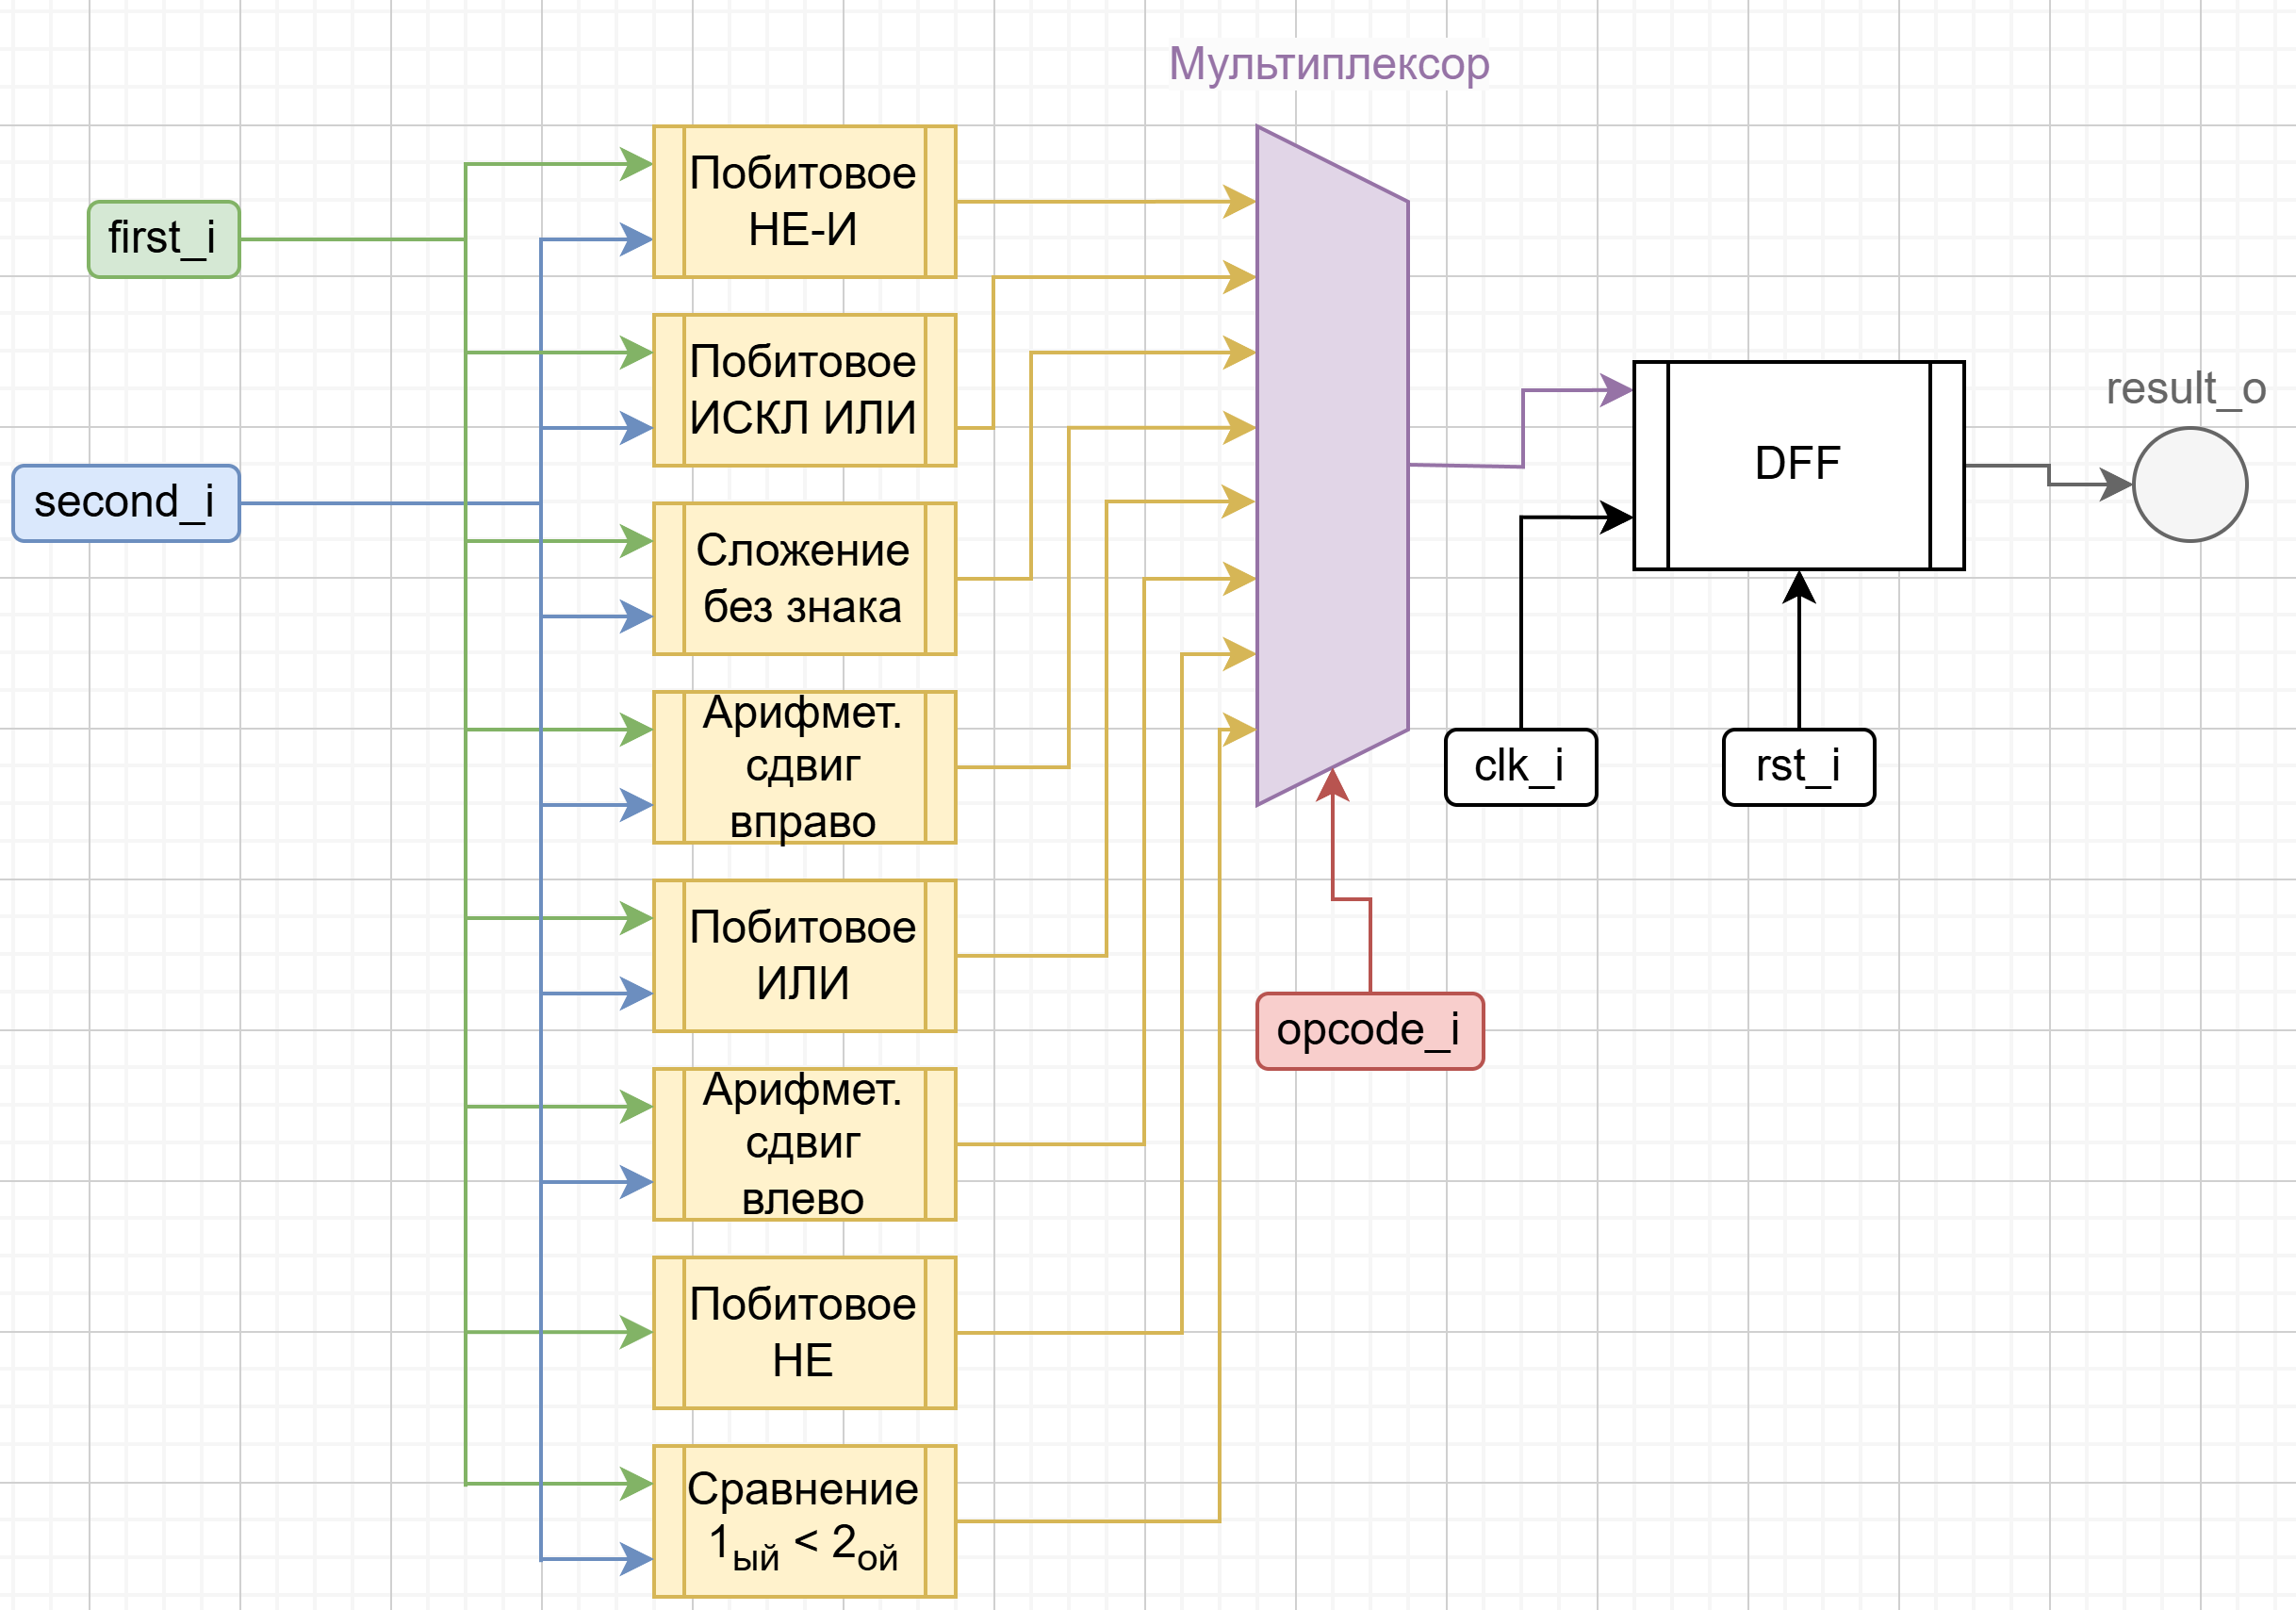
\includegraphics[width=1\linewidth]{Formal/АЛУ1.png}
\end{figure}
    \item
Параметр	WIDTH		\\
Описание	Разрядность операндов\\
Допустимые значения Целое число больше или равно 1\\
    \item
    \begin{table}[H]
\centering
\label{tab:ports}
\begin{tabular}{|l|c|l|p{6cm}|}
\hline
\textbf{Название} & \textbf{Ширина} & \textbf{Направление} & \textbf{Описание} \\ \hline
clk\_i    & 1      & Вход    & Тактовый сигнал \\ \hline
rst\_i    & 1      & Вход    & Синхронный сброс (активный уровень — 1) \\ \hline
first\_i  & WIDTH  & Вход    & Первый операнд \\ \hline
second\_i & WIDTH  & Вход    & Второй операнд \\ \hline
opcode\_i & 3      & Вход    & Код операции \\ \hline
result\_o & WIDTH  & Выход   & Результат операции \\ \hline
\end{tabular}
\end{table}
\item
Тактирование и сброс\\
Тактирование: По положительному фронту сигнала clk\_i.\\
Сброс: Синхронный (активный уровень — 1).\\
При активации rst\_i регистр обнуляется на следующем такте.
\item 
Тестирование
Сценарий тестирования:
\begin{enumerate}
\item Сброс: Проверка обнуления регистра при активации rst\_i.\\
\textbf{Проверка операций:}
\item Побитовое НЕ-И (opcode\_i = 000).
\item Исключающее ИЛИ (001).
\item Сложение (010).
\item Арифметический сдвиг вправо (011).
\item Побитовое ИЛИ (100).
\item Логический сдвиг влево (101).
\item Побитовое НЕ (110).
\item Сравнение (111).
\item Граничные случаи:
\item Переполнение при сложении.
\item Сдвиг на значение, превышающее разрядность.
\item Задержка вывода: Убедиться, что результат появляется через такт.
\item Сброс: Снова обнуление регистра.
\end{enumerate}
\item В папке будет находиться Makefile, чтобы запустить все файлы в папке, введите в консоль \textit{make run}, чтобы отчистить папку от результатов компиляции, введите \textit{make clean}.
\item
\begin{figure}[H]
    \centering
    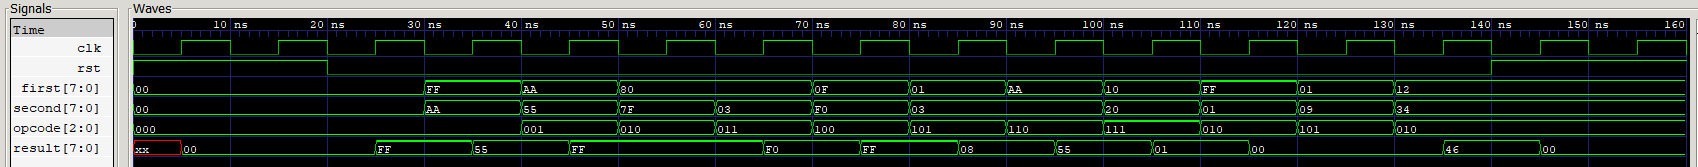
\includegraphics[width=1\linewidth]{Formal/tb.png}
\end{figure}
\end{enumerate}

\end{document}
